%%Options for presentations (in-class) and handouts (e.g. print). 
\documentclass[pdf
,handout
]{beamer}
\usepackage{pgfpages}
\pgfpagesuselayout{2 on 1}[letterpaper,border shrink=5mm]

\graphicspath{{../}}

%%%%%%%%%%%%%%%%%%%%%%
%% Change this for different slides so it appears in bar
\usepackage{authoraftertitle}
\date{Linear Transformations: Rotation Transformations in $\mathbb{R}^2$}

%%%%%%%%%%%%%%%%%%%%%%
%% Upload common style file
\usepackage{../LyryxLinearAlgebraSlidesStyle}

\begin{document}
	
	%%%%%%%%%%%%%%%%%%%%%%%
	%% Title Page and Copyright Common to All Slides
	
	%Title Page
	\input ../frontmatter/titlepage.tex
	
	%LOTS Page
	%\input frontmatter/lyryxopentexts.tex
	
	%Copyright Page
	\input ../frontmatter/copyright.tex
	
	%%%%%%%%%%%%%%%%%%%%%%%%%


\section{Rotations}

%-------------- start slide -------------------------------%
\frame{\frametitle{Recall: Matrix Transformation}
\begin{definition}
Let $A$ be an $m\times n$ matrix.  The transformation
$T:\RR^n\rightarrow\RR^m$ defined by
\[ T(\vect{x})=A\vect{x} \mbox{ for each } \vect{x}\in\RR^n\]
is called the
\alert{matrix transformation induced by $A$}.
\end{definition}

}
%---------------------end slide----------------------------%



%-------------- start slide -------------------------------%
\frame{\frametitle{Rotations in $\mathbb{R}^2$}
\begin{definition}
The transformation
\[ R_\theta: \RR^2\rightarrow \RR^2 \] denotes counterclockwise 
rotation about the origin through an angle of $\theta$.
\end{definition}
\pause
\begin{block}{}
Rotation through an angle of $\theta$ preserves
scalar multiplication.
\end{block}
\pause
\begin{block}{}
Rotation through an angle of $\theta$ preserves
vector addition.
\end{block}
}
%-------------- end slide -------------------------------%

%-------------- start slide -------------------------------%
\frame{
\begin{block}{$R_{\theta}$ is a linear transformation}
Since $R_{\theta}$ preserves addition and scalar multiplication,
$R_{\theta}$ is a linear transformation, and hence a matrix
transformation.
\bigskip

The matrix that induces $R_{\theta}$ can be found by computing
$R_{\theta}(E_1)$ and $R_{\theta}(E_2)$, where
\[ E_1=\left[\begin{array}{c} 1 \\ 0 \end{array}\right]
~\mbox{ and }
E_2=\left[\begin{array}{c} 0 \\ 1 \end{array}\right].  \]
\pause
\[ R_{\theta}(E_1)
\pause
=R_{\theta}\left[\begin{array}{r} 1 \\ 0 \end{array}\right]
\pause
=\left[\begin{array}{r} \cos\theta \\
\sin\theta \end{array}\right],\]
\pause
and
\[ R_{\theta}(E_2)
\pause
=R_{\theta}\left[\begin{array}{r} 0 \\ 1 \end{array}\right]
\pause
=\left[\begin{array}{r} -\sin\theta \\
\cos\theta \end{array}\right]\]
\end{block}
}
%-------------- end slide -------------------------------%

%-------------- start slide -------------------------------%
\frame{
\begin{block}{The Matrix for $R_{\theta}$}
The rotation $R_{\theta}:\RR^2\rightarrow\RR^2$ is a
linear transformation, and is induced by the matrix
\[ \left[\begin{array}{rr}
\cos\theta & -\sin\theta\\
\sin\theta & \cos\theta
\end{array}\right].\]
\end{block}
}
%-------------- end slide -------------------------------%


%-------------- start slide -------------------------------%
\frame{
\begin{example}[Rotation through $\pi$]
We denote by
\[ R_{\pi}:\RR^2\to\RR^2\]
counterclockwise rotation about the origin through an angle 
of $\pi$.
\pause
\begin{picture}(4,1.75)
\put(1.3,0.1){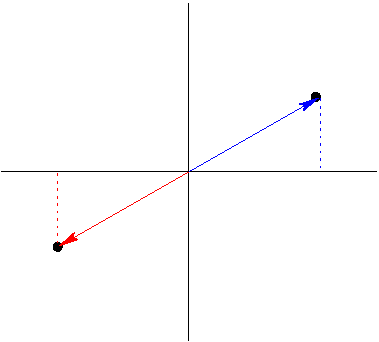
\includegraphics[scale=0.7]{figures/R2-rotate-pi.pdf}}
\put(2.25,0.75){\scriptsize{$0$}}
\put(2.05,1.6){\scriptsize{$y$}}
\put(3.0,0.75){\scriptsize{$x$}}
\put(2.85,1.22){\scriptsize{$(a,b)$}}
\pause
\put(1.0,0.5){\scriptsize{\alert{$(-a,-b)$}}}
\end{picture}
\pause

We see that $ R_{\pi}\left[\begin{array}{c} a \\ b \end{array}\right]
=
\left[\begin{array}{c} -a \\ -b \end{array}\right]
=
\pause\left[\begin{array}{rr} -1 & 0 \\ 0 & -1 \end{array}\right]
\left[\begin{array}{c} a \\ b \end{array}\right],$
so $R_{\pi}$ is a matrix transformation.
\end{example}
}
%-------------- end slide -------------------------------%

%-------------- start slide -------------------------------%
\frame{\frametitle{Rotation}
\begin{problem}\em
The transformation $ R_{\frac{\pi}{2}}:\RR^2 \rightarrow \RR^2$
denotes a \alert{counterclockwise} rotation about the origin
through an angle of $\frac{\pi}{2}$ radians. Find the matrix of $R_{\frac{\pi}{2}}$.
\end{problem}

\uncover<2->{
\begin{solution}\em
First, 
\[ R_{\frac{\pi}{2}}
\left[\begin{array}{c} a \\ b \end{array}\right]
=
\left[\begin{array}{r} -b \\ a \end{array}\right]
\]
}
\uncover<3->{Furthermore $R_{\frac{\pi}{2}}$ is a matrix
transformation, and the matrix it is induced by is 
\[ \left[\begin{array}{c} -b \\ a \end{array}\right] =
\left[\begin{array}{rr}
0 & -1 \\ 1 & 0 \end{array}\right]
\left[\begin{array}{c} a \\ b \end{array}\right]. \]}
\end{solution}
}
%-------------- end slide -------------------------------%


%-------------- start slide -------------------------------%
\frame{
\begin{example}[Rotation through $\pi/2$]
We denote by
\[ R_{\pi/2}:\RR^2\to\RR^2\]
counterclockwise rotation about the origin through an angle 
of $\pi/2$.
\pause
\begin{picture}(4,1.75)
\put(1.3,0.1){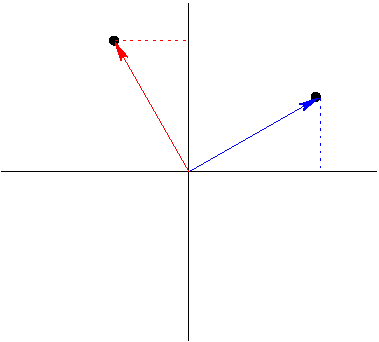
\includegraphics[scale=0.7]{figures/R2-rotate-halfpi.pdf}}
\put(2.25,0.75){\scriptsize{$0$}}
\put(2.05,1.6){\scriptsize{$y$}}
\put(3.0,0.75){\scriptsize{$x$}}
\put(2.85,1.22){\scriptsize{$(a,b)$}}
\pause
\put(1.4,1.5){\scriptsize{\alert{$(-b,a)$}}}
\end{picture}
\pause

We see that $ R_{\pi/2}\left[\begin{array}{c} a \\ b \end{array}\right]
=
\left[\begin{array}{c} -b \\ a \end{array}\right]
=
\pause\left[\begin{array}{rr} 0 & -1 \\ 1 & 0 \end{array}\right]
\left[\begin{array}{c} a \\ b \end{array}\right],$
so $R_{\pi/2}$ is a matrix transformation.
\end{example}
}
%-------------- end slide -------------------------------%


\section{Reflections}

%--------------------start slide---------------------%
\frame{\frametitle{Reflection in $\RR^2$}
\begin{example}
In $\RR^2$, reflection in the $x$-axis, which transforms 
$\left[\begin{array}{r} a \\ b \end{array}\right]$ to
$\left[\begin{array}{r} a \\ -b \end{array}\right]$, 
is a matrix transformation because
\[ \left[\begin{array}{r} a \\ -b \end{array}\right] =
\left[ \begin{array}{rr}
1 & 0 \\ 0 & -1 \end{array}\right]
\left[\begin{array}{r} a \\ b \end{array}\right].\]
\end{example}
\pause
\begin{example}
In $\RR^2$, reflection in the $y$-axis transforms 
$\left[\begin{array}{r} a \\ b \end{array}\right]$ to
$\left[\begin{array}{r} -a \\ b \end{array}\right]$.
This is a matrix transformation because
\[ \left[\begin{array}{r} -a \\ b \end{array}\right] =
\left[ \begin{array}{rr}
-1 & 0 \\ 0 & 1 \end{array}\right]
\left[\begin{array}{r} a \\ b \end{array}\right].\]
\end{example}
}
%-------------- end slide -------------------------------%

%-------------- start slide -------------------------------%
\frame{
\begin{example}
Reflection in the line $y=x$ 
transforms
$\left[\begin{array}{r} a \\ b \end{array}\right]$ to
$\left[\begin{array}{r} b \\ a \end{array}\right]$.
\bigskip

\begin{picture}(4,1.5)
\put(1.4,0){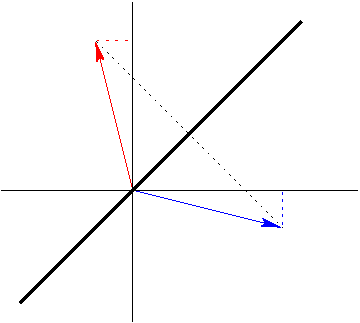
\includegraphics[scale=0.75]{figures/eigenvectors-2.pdf}}
\put(2.85,0.45){\textcolor{blue}{{\scriptsize{$(a,b)$}}}}
\put(1.55,1.4){\textcolor{red}{{\scriptsize{$(b,a)$}}}}
\put(3.2,0.63){\scriptsize{$x$}}
\put(2.1,1.5){\scriptsize{$y$}}
\put(2.8,1.3){\scriptsize{$y=x$}}
\end{picture}
\pause

This is a matrix transformation because
\[ \left[\begin{array}{r} b \\ a \end{array}\right] =
\left[ \begin{array}{rr}
0 & 1 \\ 1 & 0 \end{array}\right]
\left[\begin{array}{r} a \\ b \end{array}\right].\]
\end{example}
}
%-------------- end slide -------------------------------%



%\section{Reflection in the line}
%%-------------- start slide -------------------------------%
%\frame{
%\begin{block}{Reflection in $y=mx$ preserves scalar multiplication}
%Let $Q_m:\RR^2\rightarrow \RR^2$ denote reflection in the
%line $y=mx$, and let $\vec{u}\in\RR^2$.
%\pause
%
%\begin{picture}(4,1.5)
%\uncover<2>{
%\put(0.3,0){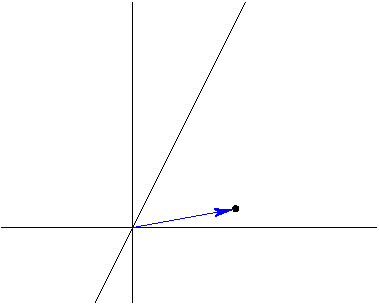
\includegraphics[scale=0.7]{figures/vectors-23a.pdf}}}
%\put(1.45,1.25){\scriptsize{$y=mx$}}
%\put(0.95,1.25){\scriptsize{$y$}}
%\put(1.95,0.25){\scriptsize{$x$}}
%\put(1.15,0.45){\scriptsize{\textcolor{blue}{$\vec{u}$}}}
%\uncover<3-5>{
%\put(0.3,0){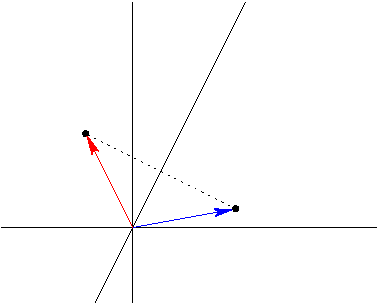
\includegraphics[scale=0.7]{figures/vectors-23b.pdf}}
%\put(0.4,0.55){\scriptsize{\textcolor{red}{$Q_m(\vec{u})$}}}
%}
%\uncover<4>{
%\put(2.5,0){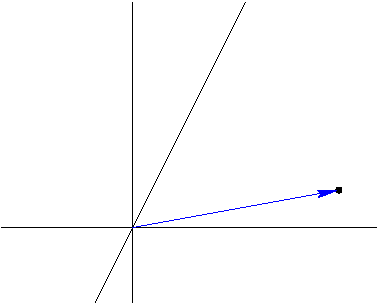
\includegraphics[scale=0.7]{figures/vectors-24a.pdf}}}
%\uncover<4->{
%\put(3.15,1.25){\scriptsize{$y$}}
%\put(4.15,0.25){\scriptsize{$x$}}
%\put(3.65,1.25){\scriptsize{$y=mx$}}
%\put(3.5,0.5){\scriptsize{\textcolor{blue}{$2\vec{u}$}}}}
%\uncover<5->{
%\put(2.5,0){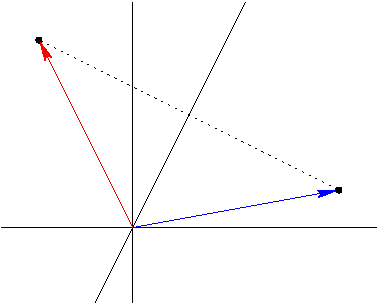
\includegraphics[scale=0.7]{figures/vectors-24.pdf}}
%\put(2.45,0.8){\scriptsize{\textcolor{red}{$Q_m(2\vec{u})$}}}}
%\uncover<6->{
%\put(0.3,0){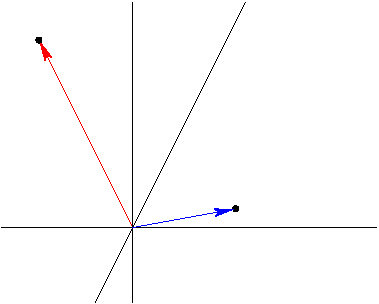
\includegraphics[scale=0.7]{figures/vectors-23.pdf}}
%\put(0.3,0.65){\scriptsize{\textcolor{red}{$2Q_m(\vec{u})$}}}
%}
%\end{picture}
%\bigskip
%
%\uncover<6->
%{The figure indicates that \alert{$Q_m(2\vec{u})=2Q_m(\vec{u})$.} }
%\uncover<7->
%{In general, for any scalar $k$, 
%\[ Q_m(kX)=kQ_m(X), \]}
%\uncover<8->
%{i.e., $Q_m$ preserves scalar multiplication.}
%\end{block}
%}
%%-------------- end slide -------------------------------%
%
%%-------------- start slide -------------------------------%
%\frame{
%\begin{block}{Reflection in $y=mx$ preserves vector addition}
%Let $\vec{u},\vec{v}\in\RR^2$.
%
%\begin{picture}(4,1.5)
%\uncover<2>{
%\put(0.3,0){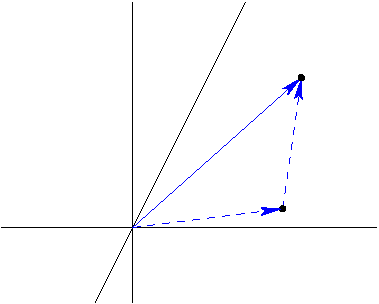
\includegraphics[scale=0.7]{figures/vectors-25a.pdf}}}
%\uncover<2->{
%\put(1.45,1.25){\scriptsize{$y=mx$}}
%\put(0.8,1.25){\scriptsize{$y$}}
%\put(1.95,0.25){\scriptsize{$x$}}
%\put(1.25,0.47){\scriptsize{\textcolor{blue}{$\vec{u}$}}}
%\put(1.7,0.7){\scriptsize{\textcolor{blue}{$\vec{v}$}}}
%\put(1.2,0.85){\scriptsize{\textcolor{blue}{$\vec{u}+\vec{v}$}}}}
%\uncover<3->{
%\put(0.3,0){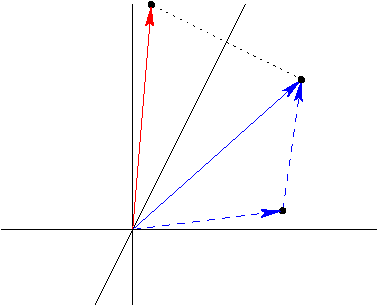
\includegraphics[scale=0.7]{figures/vectors-25.pdf}}
%\put(0.35,0.85){\scriptsize{\textcolor{red}{$Q_m(\vec{u}+\vec{v})$}}} }
%\uncover<4>{
%\put(2.5,0){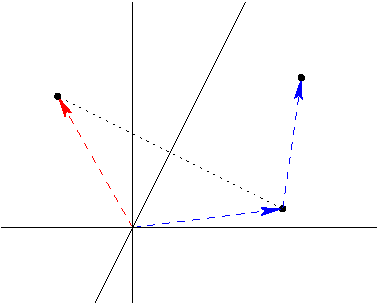
\includegraphics[scale=0.7]{figures/vectors-26a.pdf}}}
%\uncover<4->{
%\put(3.65,1.25){\scriptsize{$y=mx$}}
%\put(3.0,1.35){\scriptsize{$y$}}
%\put(4.15,0.25){\scriptsize{$x$}}
%\put(3.4,0.45){\scriptsize{\textcolor{blue}{$\vec{u}$}}}
%\put(3.9,0.7){\scriptsize{\textcolor{blue}{$\vec{v}$}}}
%\put(2.6,0.6){\scriptsize{\textcolor{red}{$Q_m(\vec{u})$}}}
%}
%\uncover<5>{
%\put(2.5,0){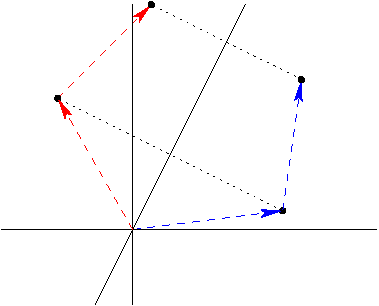
\includegraphics[scale=0.7]{figures/vectors-26b.pdf}}}
%\uncover<5->{
%\put(2.6,1.2){\scriptsize{\textcolor{red}{$Q_m(\vec{v})$}}}}
%\uncover<6->{
%\put(2.5,0){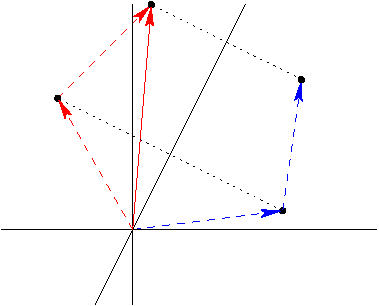
\includegraphics[scale=0.7]{figures/vectors-26c.pdf}}}
%%\uncover<7->{
%%\put(2.5,0){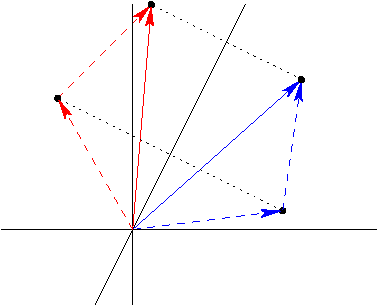
\includegraphics[scale=0.7]{figures/vectors-26.pdf}}}
%\end{picture}
%\bigskip
%
%\uncover<7->
%{The figure indicates that
%\alert{
%\[ Q_m(\vec{u}) + Q_m(\vec{v})=Q_m(\vec{u}+\vec{v}),\] } }
%\uncover<8->
%{i.e., $Q_m$ preserves vector addition.}
%\end{block}
%}
%%-------------- end slide -------------------------------%
%
%%-------------- start slide -------------------------------%
%\frame{
%\begin{block}{$Q_m$ is a linear transformation}
%Since $Q_m$ preserves addition and scalar multiplication,
%$Q_m$ is a linear transformation, and hence a matrix transformation.
%\bigskip
%\pause
%
%The matrix that induces $Q_m$ can be found by computing
%$Q_m(E_1)$ and $Q_m(E_2)$, where
%\[ 
%E_1=\left[\begin{array}{c} 1 \\ 0 \end{array}\right]
%~\mbox{ and }
%E_2=\left[\begin{array}{c} 0 \\ 1 \end{array}\right].
%\]
%\end{block}
%}
%%-------------- end slide -------------------------------%
%
%%-------------- start slide -------------------------------%
%\frame{
%\begin{block}{$Q_m(E_1)$}
%
%\begin{picture}(4,1.5)
%\uncover<1>{
%\put(1.3,0){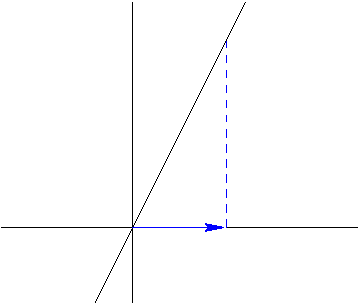
\includegraphics[scale=0.7]{figures/vectors-27a.pdf}}
%\put(2.0,0.38){\tiny{$\theta$}}}
%\uncover<1->{
%\put(2.45,1.25){\scriptsize{$y=mx$}}
%\put(1.8,1.25){\scriptsize{$y$}}
%\put(2.95,0.25){\scriptsize{$x$}} 
%\put(2.45,0.8){\scriptsize{\textcolor{blue}{$m$}}}
%\put(2.1,0.25){\scriptsize{\textcolor{blue}{$1$}}}
%}
%\uncover<2>{
%\put(1.3,0){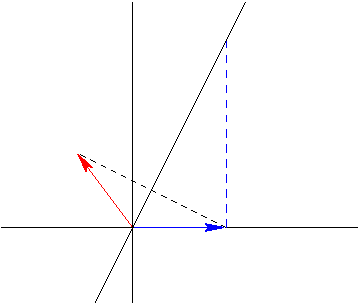
\includegraphics[scale=0.7]{figures/vectors-27b.pdf}}
%}
%\uncover<3->{
%\put(1.3,0){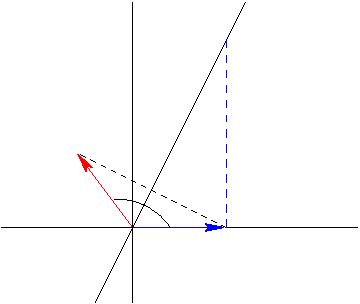
\includegraphics[scale=0.7]{figures/vectors-27c.pdf}}
%\put(2.1,0.38){\tiny{$2\theta$}}
%}
%\end{picture}
%
%\[ \cos\theta = \frac{1}{\sqrt{1+m^2}}
%~\mbox{ and }~ 
%\sin\theta = \frac{m}{\sqrt{1+m^2}} \]
%\[ \uncover<4->{
% Q_m(E_1) =\left[\begin{array}{c}
%\cos(2\theta) \\ \sin(2\theta) \end{array}\right]}
%\uncover<5->{
%=\left[\begin{array}{c}
%\cos^2\theta-\sin^2\theta \\ 2\sin\theta \cos\theta \end{array}\right]}
%\uncover<6->{
%=\frac{1}{1+m^2}\left[\begin{array}{c}
%1-m^2 \\ 2m \end{array}\right]}
%\]
%\end{block}
%}
%%-------------- end slide -------------------------------%
%
%%-------------- start slide -------------------------------%
%\frame{
%\begin{block}{$Q_m(E_2)$}
%\begin{picture}(4,1.5)
%\uncover<1>{
%\put(1.3,0){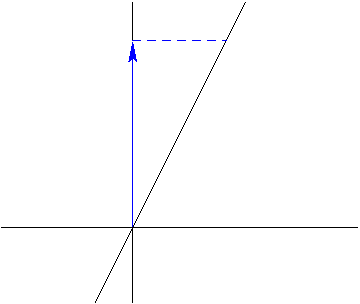
\includegraphics[scale=0.7]{figures/vectors-28a.pdf}} }
%\uncover<1->{
%\put(2.45,1.25){\scriptsize{$y=mx$}}
%\put(1.8,1.25){\scriptsize{$y$}}
%\put(2.95,0.25){\scriptsize{$x$}}
%\put(1.93,0.5){\tiny{$\theta$}}
%\put(1.75,0.8){\scriptsize{\textcolor{blue}{$1$}}}
%\put(2.1,1.35){\scriptsize{\textcolor{blue}{$\frac{1}{m}$}}}
%}
%\uncover<2>{
%\put(1.3,0){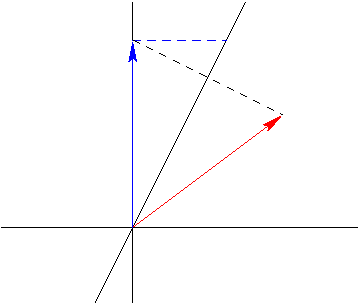
\includegraphics[scale=0.7]{figures/vectors-28b.pdf}}
%}
%\uncover<3->{
%\put(1.3,0){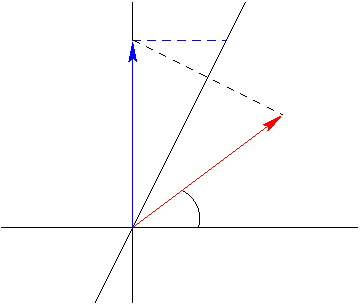
\includegraphics[scale=0.7]{figures/vectors-28c.pdf}}
%\put(2.26,0.43){\tiny{$\frac{\pi}{2}-2\theta$}} }
%\end{picture}
%
%\uncover<1->{
%\[ \cos\theta = \frac{m}{\sqrt{1+m^2}}
%~\mbox{ and }~
%\sin\theta = \frac{1}{\sqrt{1+m^2}} \]}
%\begin{eqnarray*}
%\uncover<4->{
% Q_m(E_2) & = & \left[\begin{array}{c}
%\cos(\frac{\pi}{2}-2\theta) \\ \sin(\frac{\pi}{2}-2\theta) \end{array}\right]}
%\uncover<5->{
%=\left[\begin{array}{c}
%\cos\frac{\pi}{2} \cos(2\theta)+\sin\frac{\pi}{2} \sin(2\theta) \\
%\sin\frac{\pi}{2} \cos(2\theta)-\cos\frac{\pi}{2} \sin(2\theta) \\
%\end{array}\right]} \\
%\uncover<6->{
%& = & \left[\begin{array}{c}
%\sin(2\theta) \\ \cos(2\theta) \end{array}\right]}
%\uncover<7->{
%=\left[\begin{array}{c}
%2\sin\theta \cos\theta \\ \cos^2\theta-\sin^2\theta  \end{array}\right]}
%\uncover<8->{
%=\frac{1}{1+m^2}\left[\begin{array}{c}
%2m \\ m^2-1 \end{array}\right]}
%\end{eqnarray*}
%\end{block}
%}
%%-------------- end slide -------------------------------%
%
%%-------------- start slide -------------------------------%
%\frame{
%\begin{block}{The Matrix for Reflection in $y=mx$}
%The transformation $Q_m:\RR^2\rightarrow\RR^2$,
%reflection in the line $y=mx$,
%is a linear transformation and is induced by the matrix
%\[ \frac{1}{1+m^2} 
%\left[\begin{array}{cc}
%1-m^2 & 2m \\ 2m & m^2-1
%\end{array}\right].\]
%\end{block}
%}
%%-------------- end slide -------------------------------%
%
%%-------------- start slide -------------------------------%
%\frame{\frametitle{Multiple Actions}
%\begin{problem}\em
%Find the rotation or reflection that equals reflection in the
%$x$-axis followed by rotation through an angle of $\frac{\pi}{2}$.
%\end{problem}
%
%\uncover<2->{
%\begin{solution}\em
%Let $Q_0$ denote the reflection in the $x$-axis, and $R_{\frac{\pi}{2}}$ denote the rotation through an angle of $\frac{\pi}{2}$. We want to find the matrix for the transformation
%$R_{\frac{\pi}{2}}\circ Q_0$.}
%
%\uncover<3->{
%$Q_0$ is induced by
%$A= \left[\begin{array}{rr}
%1 & 0 \\ 0 & -1
%\end{array}\right]$, and
%$R_{\frac{\pi}{2}}$ is induced by
%\[
%B=\left[\begin{array}{rr}
%\cos\frac{\pi}{2} & -\sin\frac{\pi}{2} \\
%\sin\frac{\pi}{2} & \cos\frac{\pi}{2}
%\end{array}\right]
%=
%\left[\begin{array}{rr}
%0 & -1 \\ 1 & 0
%\end{array}\right]
%\]}
%\end{solution}
%}
%%------------------end slide-------------------%
%
%%-------------------start slide--------------%
%\frame{
%\begin{solution}\em
%Hence $R_{\frac{\pi}{2}}\circ Q_0$ is induced by 
%\[ BA = 
%\left[\begin{array}{rr}
%0 & -1 \\ 1 & 0
%\end{array}\right]
%\left[\begin{array}{rr}
%1 & 0 \\ 0 & -1
%\end{array}\right]
%=
%\left[\begin{array}{rr}
%0 & 1 \\ 1 & 0
%\end{array}\right].\]
%
%\pause
%
%Notice that
%$BA= \left[\begin{array}{rr}
%0 & 1 \\ 1 & 0
%\end{array}\right]$
%is a \alert{reflection} matrix.
%
%\pause
%\begin{center}
%\alert{\Large How do we know this?}
%\end{center}
%
%\end{solution}
%}
%%-----------------end slide---------------%
%
%%-------------------start slide-------------%
%\frame{
%\begin{solution}[continued]\em
%
%Compare $BA$ to 
%\[ Q_m = \frac{1}{1+m^2}
%\left[\begin{array}{cc}
%1-m^2 & 2m \\ 2m & m^2-1
%\end{array}\right]
%\]
%
%
%\uncover<2->{
%Now, since $1-m^2=0$, we know that $m=1$ or $m=-1$.  
%But $\frac{2m}{1+m^2}=1>0$, so $m>0$, implying $m=1$.}
%\medskip
%
%\uncover<3->{
%Therefore, 
%\[ R_{\frac{\pi}{2}}\circ Q_0 = Q_1,\]
%reflection in the line $y=x$.}
%\end{solution}
%}
%%-------------- end slide -------------------------------%
%
%%-------------- start slide -------------------------------%
%\frame{\frametitle{Reflection followed by Reflection}
%\begin{problem}\em
%Find the rotation or reflection that equals reflection in the
%line $y=-x$ followed by reflection in the $y$-axis.
%\end{problem}
%
%\uncover<2->{
%\begin{solution}\em
%We must find the matrix for the transformation
%$Q_Y\circ Q_{-1}$.}
%\bigskip
%
%\uncover<3->{
%$Q_{-1}$ is induced by
%\[ A= \frac{1}{2}\left[\begin{array}{rr}
%0 & -2 \\ -2 & 0
%\end{array}\right]
%=
%\left[\begin{array}{rr}
%0 & -1 \\ -1 & 0
%\end{array}\right],
%\]
%and
%$Q_{Y}$ is induced by
%\[
%B=\left[\begin{array}{rr}
%-1 & 0 \\ 0 & 1
%\end{array}\right].
%\]}
%
%\uncover<4->{
%Therefore, $Q_Y\circ Q_{-1}$ is induced by $BA$.
%}
%\end{solution}
%}
%%-------------- end slide -------------------------------%
%
%%-------------- start slide -------------------------------%
%\frame{
%\begin{solution}[continued]\em
%\[ BA = \left[\begin{array}{rr}
%-1 & 0 \\ 0 & 1
%\end{array}\right]
%\left[\begin{array}{rr}
%0 & -1 \\ -1 & 0
%\end{array}\right]
%=
%\left[\begin{array}{rr}
%0 & 1 \\ -1 & 0
%\end{array}\right].\]
%\medskip
%
%\uncover<2->{
%\begin{center}
%\alert{\Large What transformation does $BA$ induce?}
%\end{center} }
%\medskip
%
%\uncover<3->{
%Rotation through an angle $\theta$ such that
%\[ \cos\theta = 0 \mbox{ and } \sin\theta = -1.\]
%}
%\medskip
%
%\uncover<4->{
%Therefore, $Q_Y\circ Q_{-1} = R_{-\frac{\pi}{2}} = 
%R_{\frac{3\pi}{2}}$.}
%\end{solution}
%}
%%-------------- end slide -------------------------------%
%
%%-------------- start slide -------------------------------%
%\frame{\frametitle{Summary}
%In general,
%\begin{itemize}
%\item The composite of two rotations is a \pause rotation
%\[
%R_\theta\circ R_\eta=R_{\theta+\eta}
%\]
%\pause
%\item <2-> The composite of two reflections is a \pause rotation.
%\[
%Q_m\circ Q_n = R_{\theta}
%\]
%where $\theta$ is $2\times$ the  angle between lines $y=mx$ and $y=nx$. 
%\bigskip
%\pause
%\item<3-> The composite of a reflection and a rotation is a \pause
%reflection.
%\[
%R_{\theta}\circ Q_n
%= 
%Q_m\circ Q_n\circ Q_n  
%=Q_m
%\]
%\end{itemize}
%}
%%-------------- end slide -------------------------------%

\end{document}
